\chapter{Interface et valorisation opérationnelle}
\label{chapitre:interface}

L'interface de priorisation occupe ce chapitre. Le besoin opérationnel et les principes de
conception qui en découlent ouvrent l'exposé, suivis du tableau de bord et de ses trois
échelles de lecture. Les niveaux de priorité et l'action associée viennent ensuite, puis
l'export et la traçabilité des alertes, avant la portée et les limites de cet usage.

% =====================================================================
\section{Besoin opérationnel et principes de conception}
% =====================================================================
Comme précédemment mentionné au Chapitre~\ref{chapitre:contexte}, l'observation humaine
reste la référence du repérage de la boiterie, mais elle est difficile
à maintenir de façon régulière sur l'ensemble d'un troupeau, par le temps qu'elle demande et
par la variabilité entre observateurs. Les branches de détection
décrites au Chapitre~\ref{chapitre:systeme} produisent un score, des épisodes et des
notifications. Sous cette formule, ces sorties répondent
à la question « que dit le détecteur~? », alors que la question de terrain est la suivante~:
« quelles vaches dois-je aller voir aujourd'hui, et pourquoi~? ». L'interface graphique
proposée comble cet écart en transformant des séries de sortie en une liste ordonnée de
vaches à vérifier. Sa conception suit quatre principes, qui découlent du positionnement
retenu pour le système.
\begin{itemize}
  \item \emph{La priorisation plutôt que le diagnostic}. L'interface ordonne les
  vaches à observer, sans quantifier réellement une probabilité de boiterie ou afficher un
  libellé clinique. Cette contrainte est délibérée~: le corpus principal ne comporte pas
  d'étalon vétérinaire, et un affichage qui suggérerait une conclusion clinique dépasserait ce
  que les données autorisent \citep{alsaaod2019automatic}.

  \item \emph{La traçabilité de chaque alerte}. La vue individuelle présente les
  signaux, les épisodes et les notifications d'une même vache, de sorte qu'une priorité
  affichée peut toujours être remontée jusqu'aux mesures qui l'ont produite. Une alerte
  opaque serait inutilisable en ferme. L'éleveur doit alors pouvoir juger lui-même si le
  comportement observé justifie un déplacement.

  \item \emph{La séparation entre surveillance et vérification}. Une instabilité
  isolée n'appelle pas le même geste qu'une hypoactivité persistante. L'interface conserve
  cette distinction au lieu de fondre les deux branches en un signal similaire, ce qui évite de
  transformer une piste exploratoire en consigne de travail.

  \item \emph{L'absence de logique d'alerte parallèle}. L'interface lit les sorties
  du noyau de détection et ne recalcule aucune règle qui lui serait propre. Une modification de
  présentation ne peut donc pas changer silencieusement les résultats rapportés
  \citep{sculley2015hidden}.
\end{itemize}

% =====================================================================
\section{Tableau de bord de priorisation}
\label{sec:interface_streamlit}
% =====================================================================
L'interface proposée est un outil de lecture et de priorisation. Elle charge par défaut le
fichier d'entrée \texttt{data/brut.csv} et accepte un CSV importé
(Figure~\ref{fig:streamlit_overview}). La vue troupeau ordonne
les vaches à vérifier tandis que la carte thermique permet une comparaison journalière. La
méthode IF est toujours sollicitée comme comparateur qui ne constitue pas la notification
principale.

La barre latérale regroupe le chargement des données et les paramètres de calcul, tandis que
l'en-tête rappelle la source analysée, son volume et son empreinte. Les six compteurs
résument, pour la vache sélectionnée, le nombre d'intervalles analysés puis fusionnés, les
anomalies du comparateur, les candidats de chaque branche et les notifications retenues.

\begin{figure}[H]
  \centering
  % La capture fait 2878 px de large : a 0,98 de la largeur du texte, soit
  % 6,40 pouces, elle rend a 450 ppp, tres au-dessus du seuil d'impression. Le
  % rapport large et bas de la vue tient en une demi-page en portrait.
  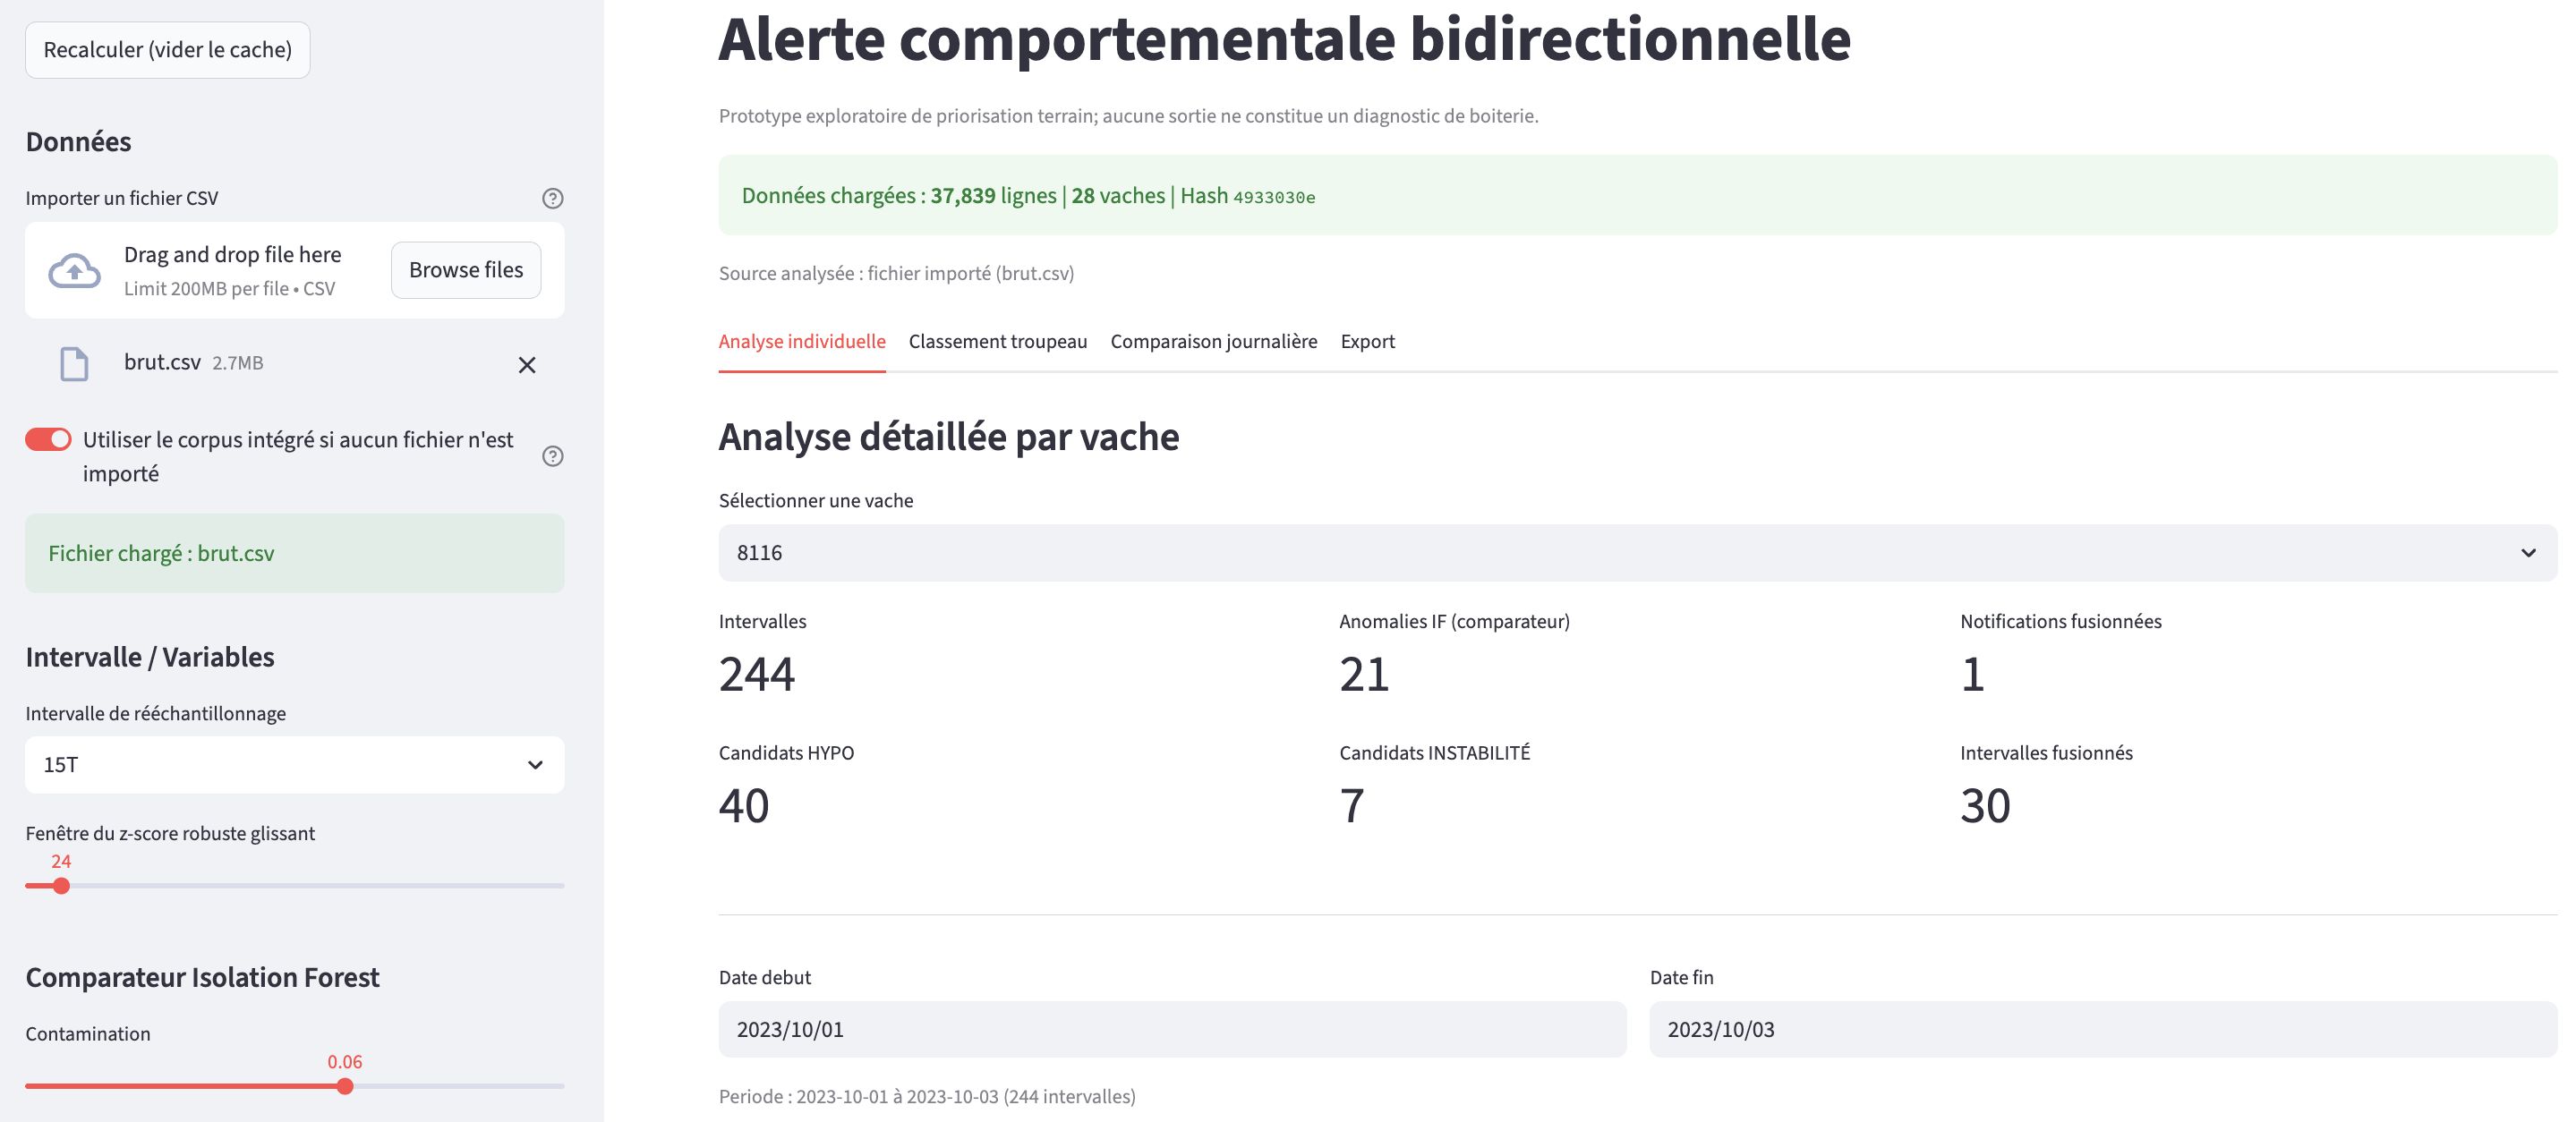
\includegraphics[width=0.98\textwidth]{figures/streamlit_overview.png}
  \caption{Vue d'ensemble du tableau de bord.}
  \label{fig:streamlit_overview}
\end{figure}

Les Figures~\ref{fig:streamlit_individual} à~\ref{fig:streamlit_heatmap} montrent comment une
même alerte est examinée à trois échelles complémentaires~: 1-~les signaux d'une vache,
2-~son rang dans le troupeau et 3-~la distribution journalière des alertes. Les marqueurs
localisent les intervalles à examiner, le classement et la carte thermique organisent l'ordre
de vérification.

Sur une fenêtre de trois jours, la vue individuelle superpose les variables retenues à
l'affichage~: l'indice de mouvement, les pas et le temps couché. Dans la
Figure~\ref{fig:streamlit_individual}, la légende nomme ces marqueurs~: \emph{Anomalie IF} en
bleu-vert, \emph{Épisode HYPO} en rouge, \emph{Épisode INSTABILITÉ} en ambre et
\emph{Notification} pour l'étoile violette qui ouvre l'épisode. Superposer ces marqueurs aux signaux bruts permet de
vérifier qu'une notification s'appuie sur une dégradation étendue dans le temps plutôt que
sur une valeur isolée. Les anomalies du comparateur restent affichées à titre de repère~;
elles ne déclenchent aucune notification.

% Page paysage, meme dispositif que la figure des vaches a verifier et que
% celle du chapitre 6 : trois panneaux superposes sur trois jours restent
% denses a la largeur du texte, la vue pivotee leur donne un tiers de largeur
% en plus. Le folio normal tomberait sur le bord gauche une fois la page
% pivotee, on le neutralise et on le replace, pivote, au bas de la vue.
\begin{landscape}
  \thispagestyle{empty}%
  \AddToShipoutPictureFG*{%
    \AtPageLowerLeft{\raisebox{0.5\paperheight}{\makebox[\paperwidth][r]{%
      \rotatebox{90}{\makebox[0pt][c]{\thepage}}\hspace{1.9cm}}}}%
  }%
  \vspace*{\fill}
  \begin{figure}[H]
    \centering
    % La capture fait 2582 px. Etalee sur 0,99 de la ligne en paysage, soit
    % 8,94 pouces, elle rend a 289 ppp, juste sous le seuil d'impression usuel
    % mais sans perte visible a cette taille de trait. Le paysage gagne en
    % echange un tiers de largeur.
    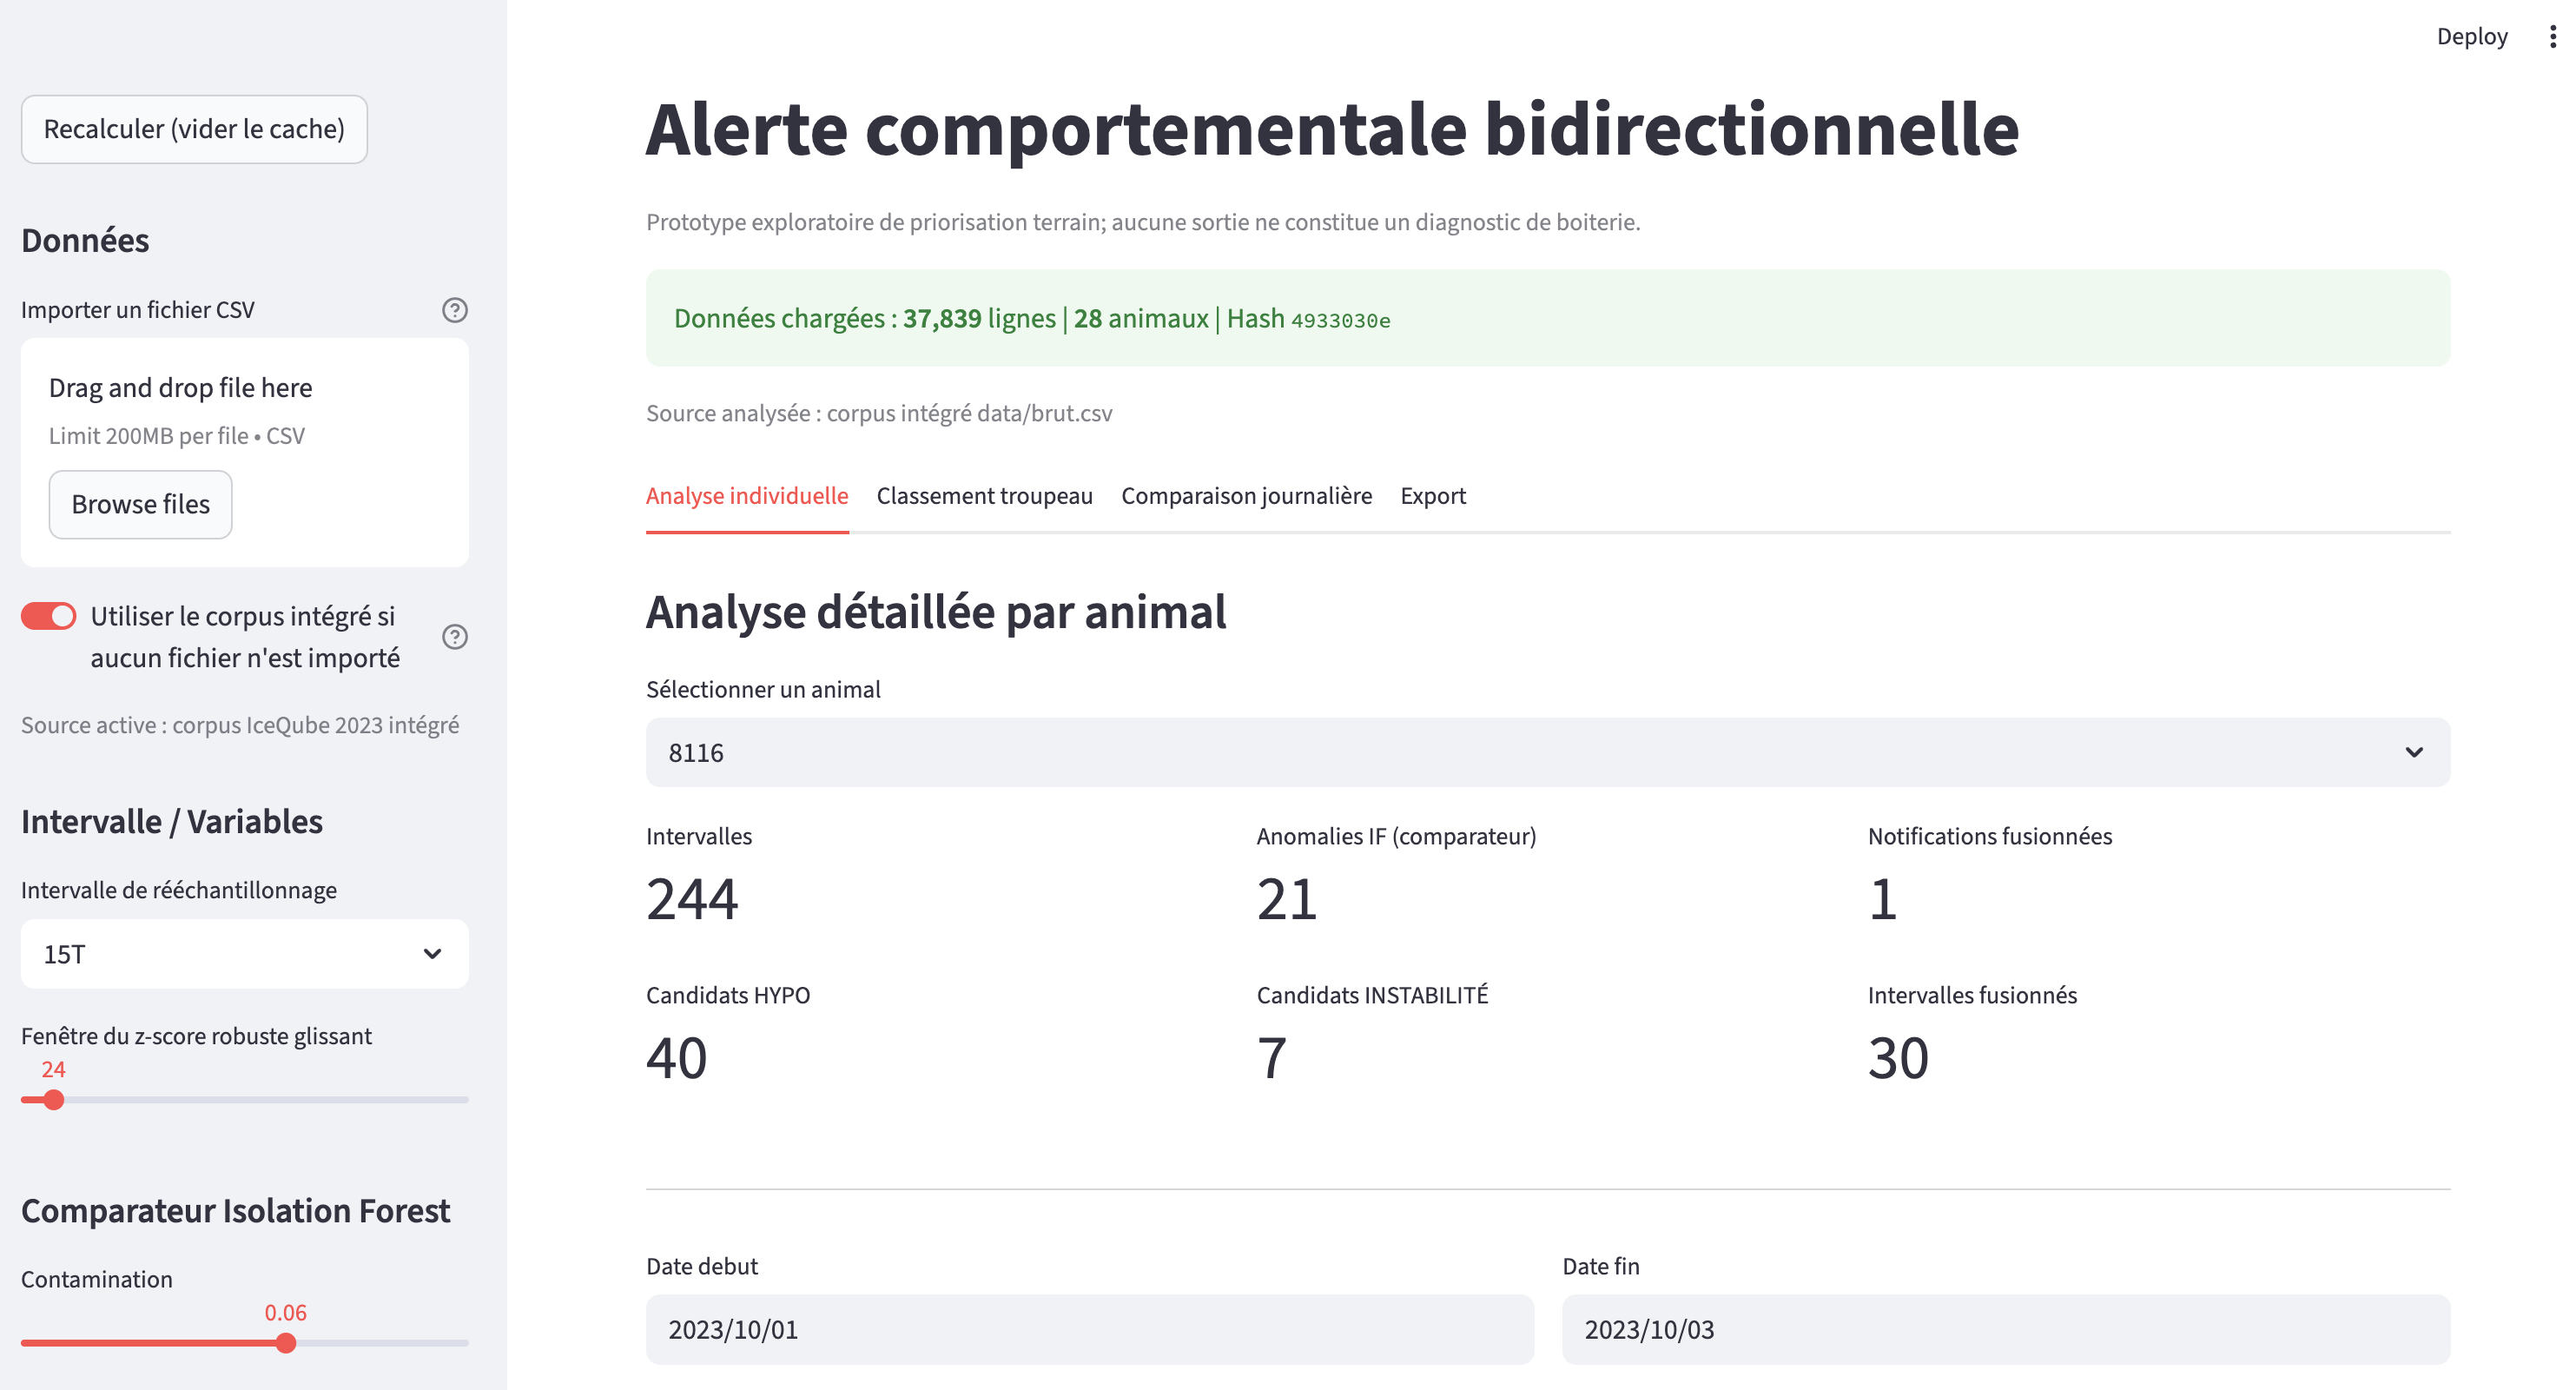
\includegraphics[width=0.99\linewidth]{figures/streamlit_individual.png}
    \caption{Analyse individuelle du tableau de bord.}
    \label{fig:streamlit_individual}
  \end{figure}
  \vfill
\end{landscape}

Le classement ordonne ensuite les vaches exploitables par priorité de vérification
(Figure~\ref{fig:streamlit_herd_table}). La colonne de rang donne l'ordre dans lequel les
aborder, tandis que les colonnes HYPO et INSTABILITÉ séparent les deux branches à l'origine
des notifications fusionnées~: un même rang peut provenir d'une hypoactivité persistante ou
d'une instabilité isolée, ce que le seul décompte fusionné ne dirait pas. Les colonnes de
couverture qualifient la fiabilité de la donnée sous-jacente~; un rang élevé associé à une
couverture faible appelle d'abord une vérification du capteur avant une observation de
la vache. La colonne d'anomalies Isolation Forest y figure au même titre que dans la vue
individuelle, comme comparateur.

\begin{figure}[H]
  \centering
  % La capture des vingt-huit rangs fait 1992 px de large : a 0,98 de la
  % largeur du texte, soit 6,40 pouces, elle rend a 311 ppp. La largeur maximale
  % est prise a dessein, ce tableau etant celui dont le corps se reduit le plus
  % une fois ramene a la page.
  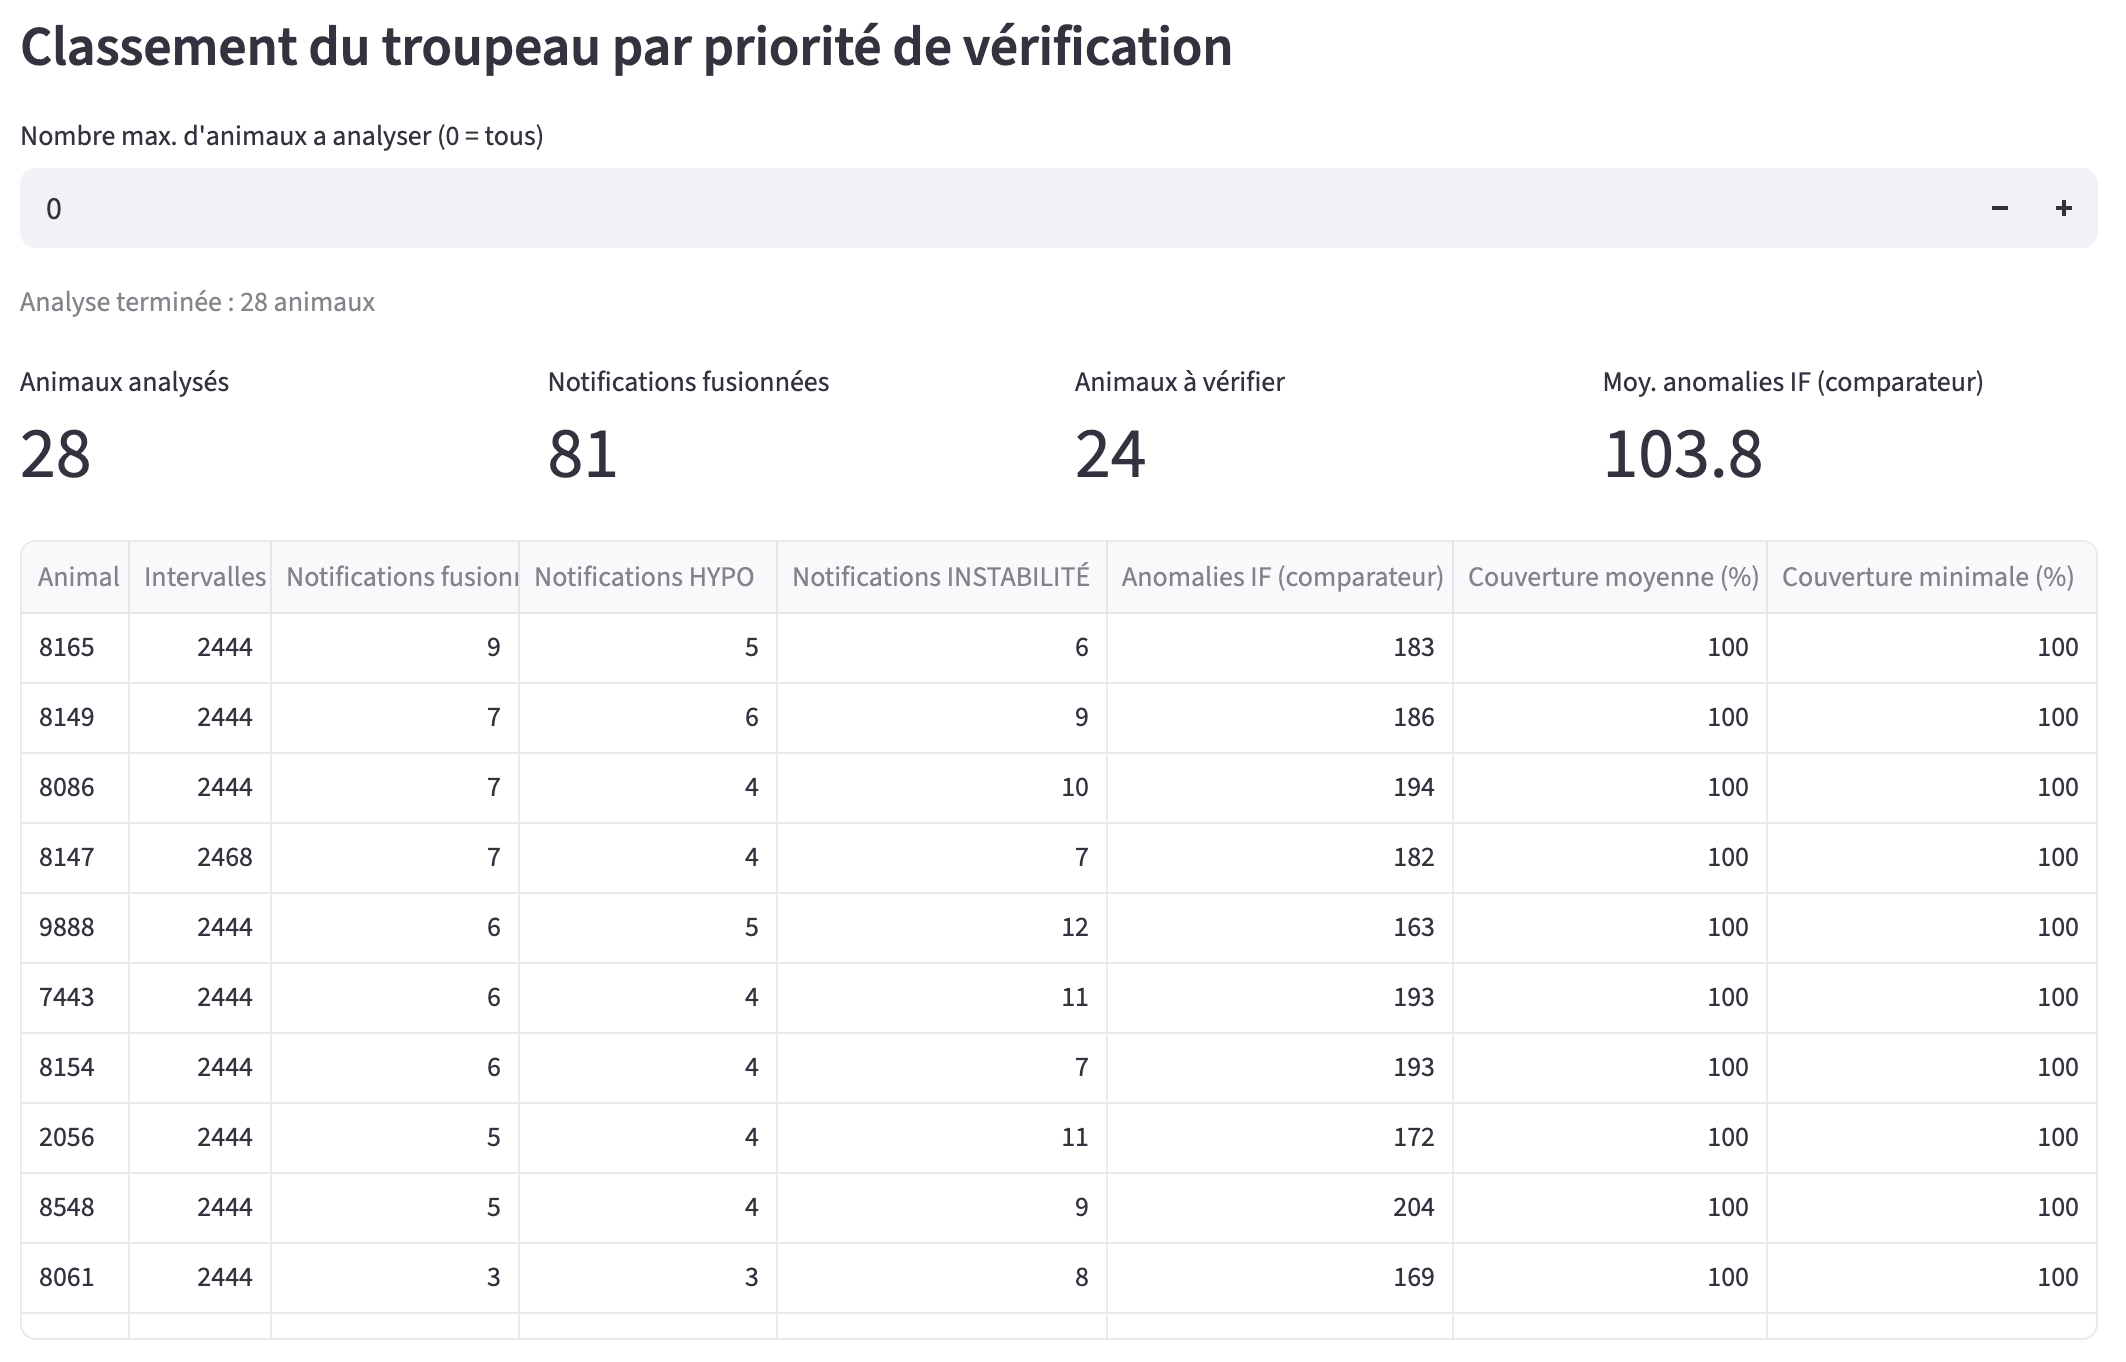
\includegraphics[width=0.98\textwidth]{figures/streamlit_herd_table.png}
  \caption{Onglet de classement du troupeau par priorité de vérification.}
  \label{fig:streamlit_herd_table}
\end{figure}

Chaque ligne de la Figure~\ref{fig:streamlit_heatmap} correspond enfin à une vache, chaque
colonne à une journée, et l'intensité traduit la sévérité des alertes de la journée. Cette
lecture déplace le regard de la vache vers le troupeau et fait apparaître des regroupements
qu'un classement cumulé masque~: une suite de journées consécutives sur une même vache ne se
lit pas comme quelques journées dispersées, et plusieurs vaches alertées le même jour
orientent vers une cause commune, de conduite ou de logement, plutôt que vers un problème
individuel. Les journées et les vaches sans mesure y restent grises, une absence de donnée
n'étant pas une absence d'alerte. La courbe placée dessous donne le nombre de vaches en alerte
et celui des vaches observées.

\begin{figure}[H]
  \centering
  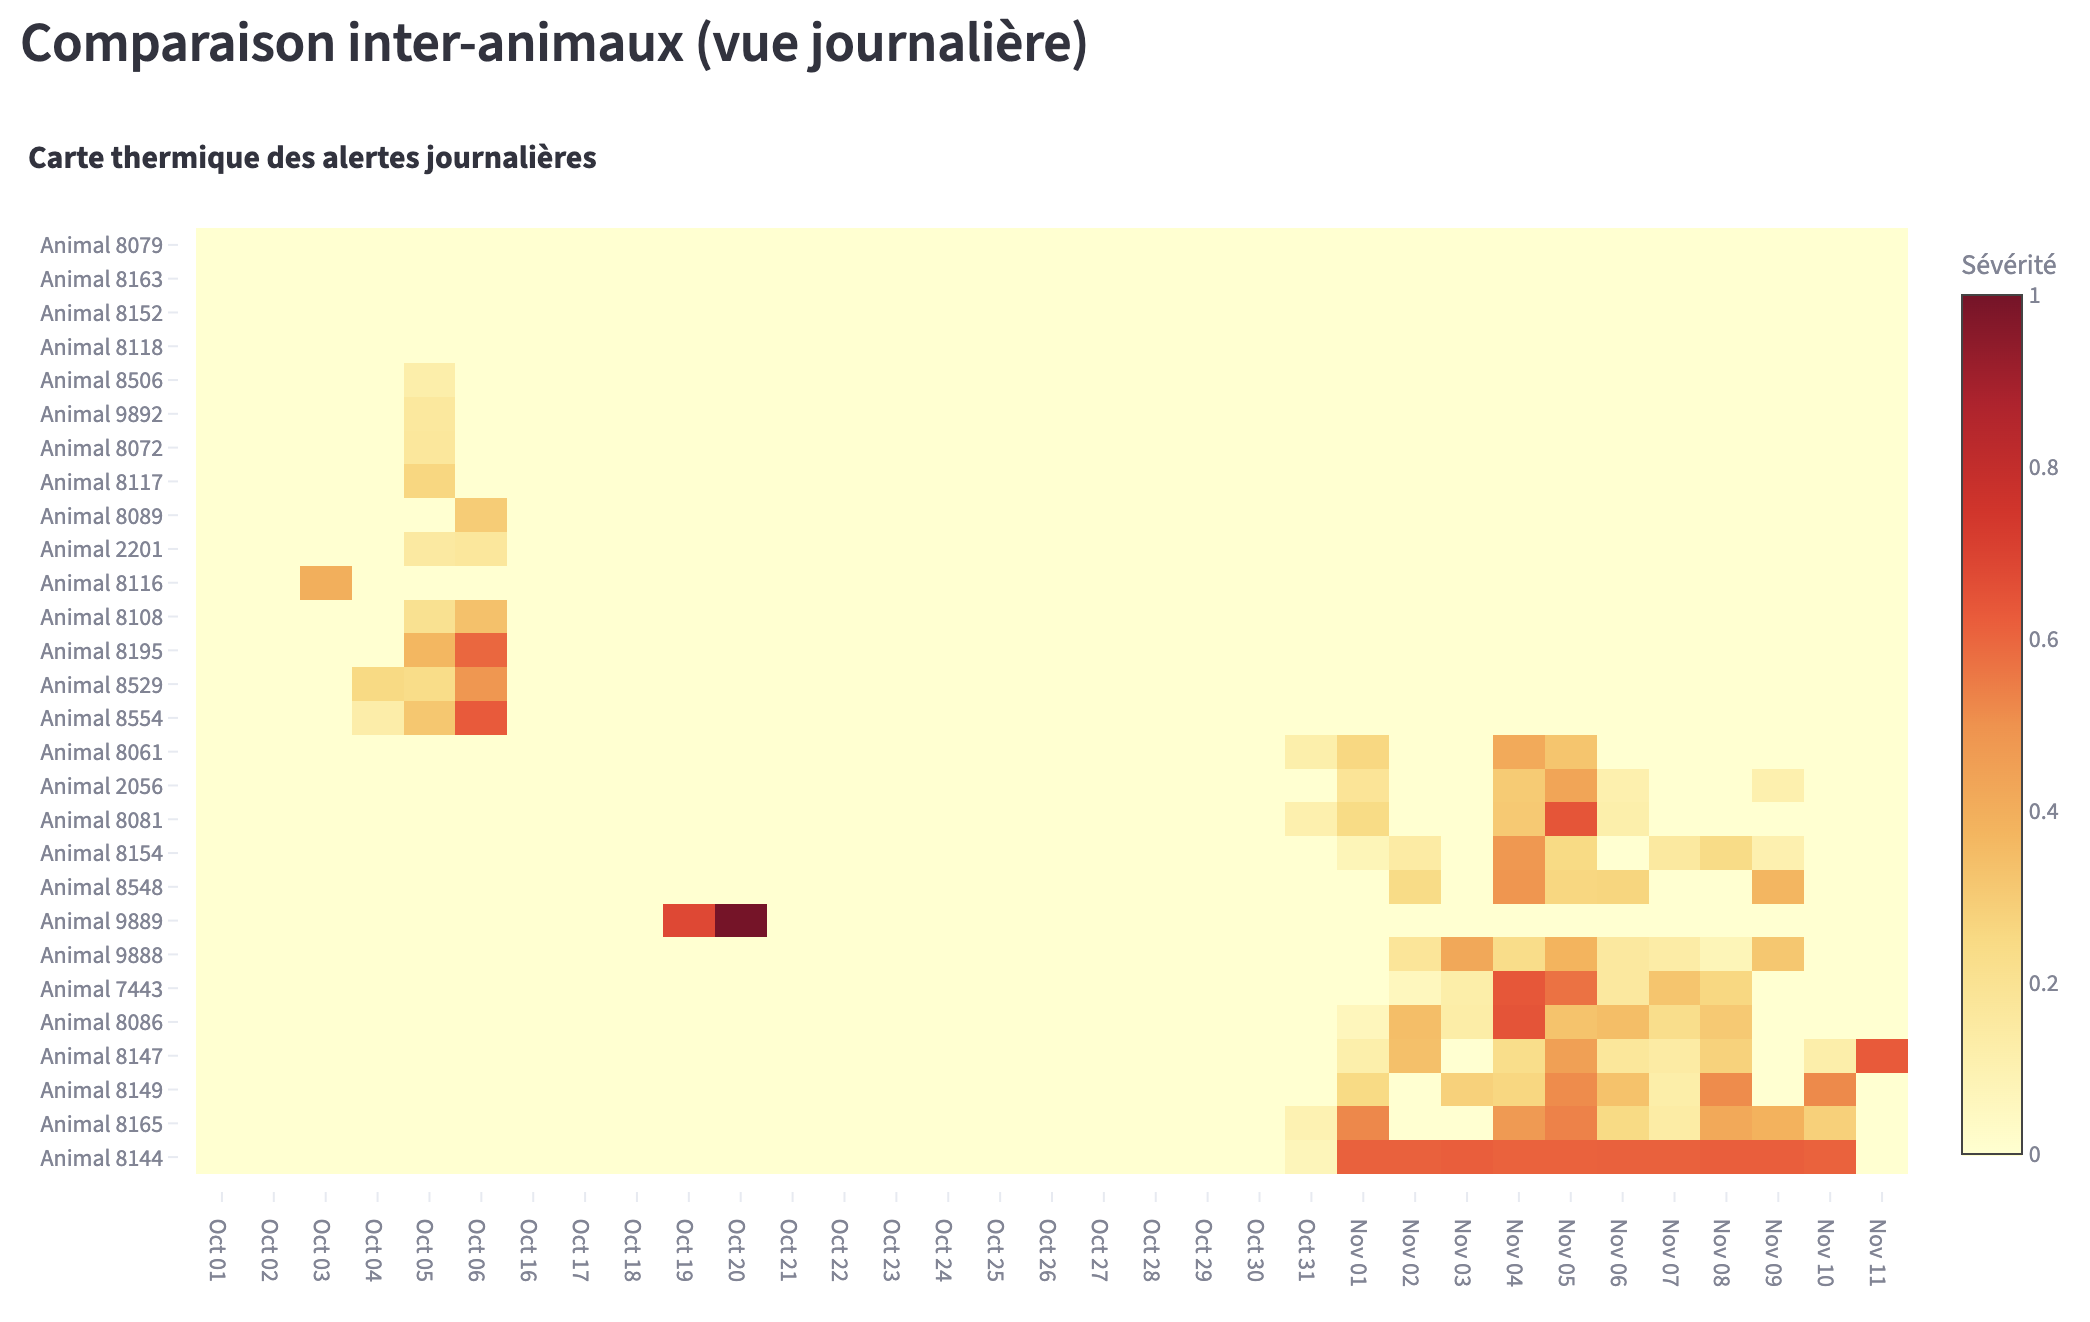
\includegraphics[width=0.98\textwidth]{figures/streamlit_heatmap_compact.png}
  \caption{Alertes journalières par vache et effectifs quotidiens du troupeau.}
  \label{fig:streamlit_heatmap}
\end{figure}

% =====================================================================
\section{Niveaux de priorité et action associée}
% =====================================================================
L'interface traduit la sortie de fusion en trois niveaux de priorité qui orientent l'effort
de vérification, comme le montre le Tableau~\ref{tab:priorites}. Seules les
priorités~2 et~3 produisent une notification de vérification~; la priorité~1 reste un signal de
surveillance.

Le choix de trois niveaux discrets, plutôt que d'un score continu, tient à la décision qu'ils
doivent servir. Sur le terrain, la question n'est pas de comparer des dixièmes entre deux
vaches, mais de trancher entre trois gestes~: se déplacer aujourd'hui, planifier une
observation, ou ne rien faire. Trois niveaux couvrent exactement ces trois issues. Un score
continu, lui, suggérerait une finesse de discrimination que les données n'autorisent pas~:
le corpus principal ne comporte aucun étalon vétérinaire qui permettrait de calibrer une
échelle, et afficher deux décimales reviendrait à donner du crédit à des écarts que rien ne
valide.

Ces niveaux reprennent directement la règle de fusion hiérarchique décrite au
Chapitre~\ref{chapitre:systeme}, sans la réinterpréter. La priorité~3 correspond aux
situations où les deux branches concordent, par convergence simultanée ou par séquence~: le
comportement s'y écarte de plusieurs manières à la fois, ce qui rend l'écart plus difficile à
attribuer au hasard ou à un artefact de mesure. La priorité~2 correspond à une hypoactivité
persistante seule, la branche dont le Chapitre~\ref{chapitre:resultats} montre qu'elle est la
mieux étayée. La priorité~1 correspond à une instabilité isolée, tenue à distance de la
notification tant qu'aucune baisse d'activité ne l'accompagne.

\begin{table}[H]
  \centering
  \caption{Niveaux de priorité de l'interface et action de vérification associée.}
  \label{tab:priorites}
  \small
  \begin{tabular}{cp{0.36\textwidth}p{0.38\textwidth}}
    \toprule
    Priorité & Condition & Action suggérée \\
    \midrule
    3 & Convergence HYPO + INSTABILITÉ, ou séquence instabilité$\rightarrow$hypoactivité &
    Vérification rapprochée, observation locomotrice \\
    2 & Hypoactivité persistante (HYPO) & Vérification à planifier \\
    1 & Instabilité isolée & Surveillance, sans alerte de vérification \\
    \bottomrule
  \end{tabular}
\end{table}

Cette gradation traduit une asymétrie de coût plutôt qu'une échelle de gravité. Un déplacement
inutile coûte quelques minutes~; une dégradation ignorée coûte du temps d'évolution, et c'est
précisément ce temps que la détection précoce cherche à récupérer. Les priorités~2 et~3
déclenchent donc une notification, quitte à ce qu'une part d'entre elles ne débouche sur rien.
La priorité~1, à l'inverse, se contente d'attirer l'attention~: elle signale une situation à
regarder si l'occasion se présente, sans imposer de geste ni entrer dans le décompte des
vérifications à effectuer. Séparer ces deux régimes évite qu'une piste exploratoire, dont le
lien avec la boiterie reste à établir, ne se transforme en charge de travail quotidienne.

Une même situation ne remonte pas indéfiniment~: une période réfractaire suit chaque
notification, de sorte qu'un épisode qui se prolonge apparaît une fois plutôt que d'occuper la
liste à chaque intervalle. Ce mécanisme, décrit au Chapitre~\ref{chapitre:systeme}, importe
autant que le seuil lui-même~: sans lui, une seule vache en dégradation lente saturerait le
classement et masquerait les autres.

À l'écran, chaque vache retenue est accompagnée du décompte de ses notifications fusionnées,
HYPO et INSTABILITÉ, et d'une vignette qui situe ses épisodes dans la période observée, comme
le représente la Figure~\ref{fig:streamlit_priority_animals}. L'ordre de vérification et le
motif qui le justifie se lisent ainsi ensemble, sans qu'il soit nécessaire de revenir à la
vue individuelle de chaque vache.

% Page paysage. Six vignettes sur deux colonnes restent illisibles a la largeur
% du texte : la vue pivotee leur donne un quart de largeur en plus, et c'est la
% lisibilite qui prime ici sur la finesse d'impression. Meme
% dispositif qu'au chapitre 6 : le folio normal tomberait sur le bord gauche
% une fois la page pivotee, on le neutralise et on le replace, pivote, au bas
% de la vue.
\begin{landscape}
  \thispagestyle{empty}%
  \AddToShipoutPictureFG*{%
    \AtPageLowerLeft{\raisebox{0.5\paperheight}{\makebox[\paperwidth][r]{%
      \rotatebox{90}{\makebox[0pt][c]{\thepage}}\hspace{1.9cm}}}}%
  }%
  % Ressorts elastiques de part et d'autre : la figure se cale au milieu de la
  % hauteur de page au lieu de rester en haut, le blanc se repartissant alors
  % egalement au-dessus et au-dessous.
  \vspace*{\fill}
  \begin{figure}[H]
    \centering
    % 0,96 et non 0,98 : la capture fait 2526 px pour un rapport de 1,56, si bien
    % qu'a 0,98 la figure et sa legende depasseraient la hauteur disponible. Un
    % depassement de trois dixiemes de point suffit ici a repousser le flottant
    % et a ajouter une page. A 0,96 elle occupe 5,55 pouces sur 8,67 de large et
    % rend a 291 ppp, juste sous le seuil usuel mais sans perte visible sur un
    % trace au trait. La largeur reste prise au plus haut : les graduations et
    % les dates des vignettes ne se lisent qu'a cette taille.
    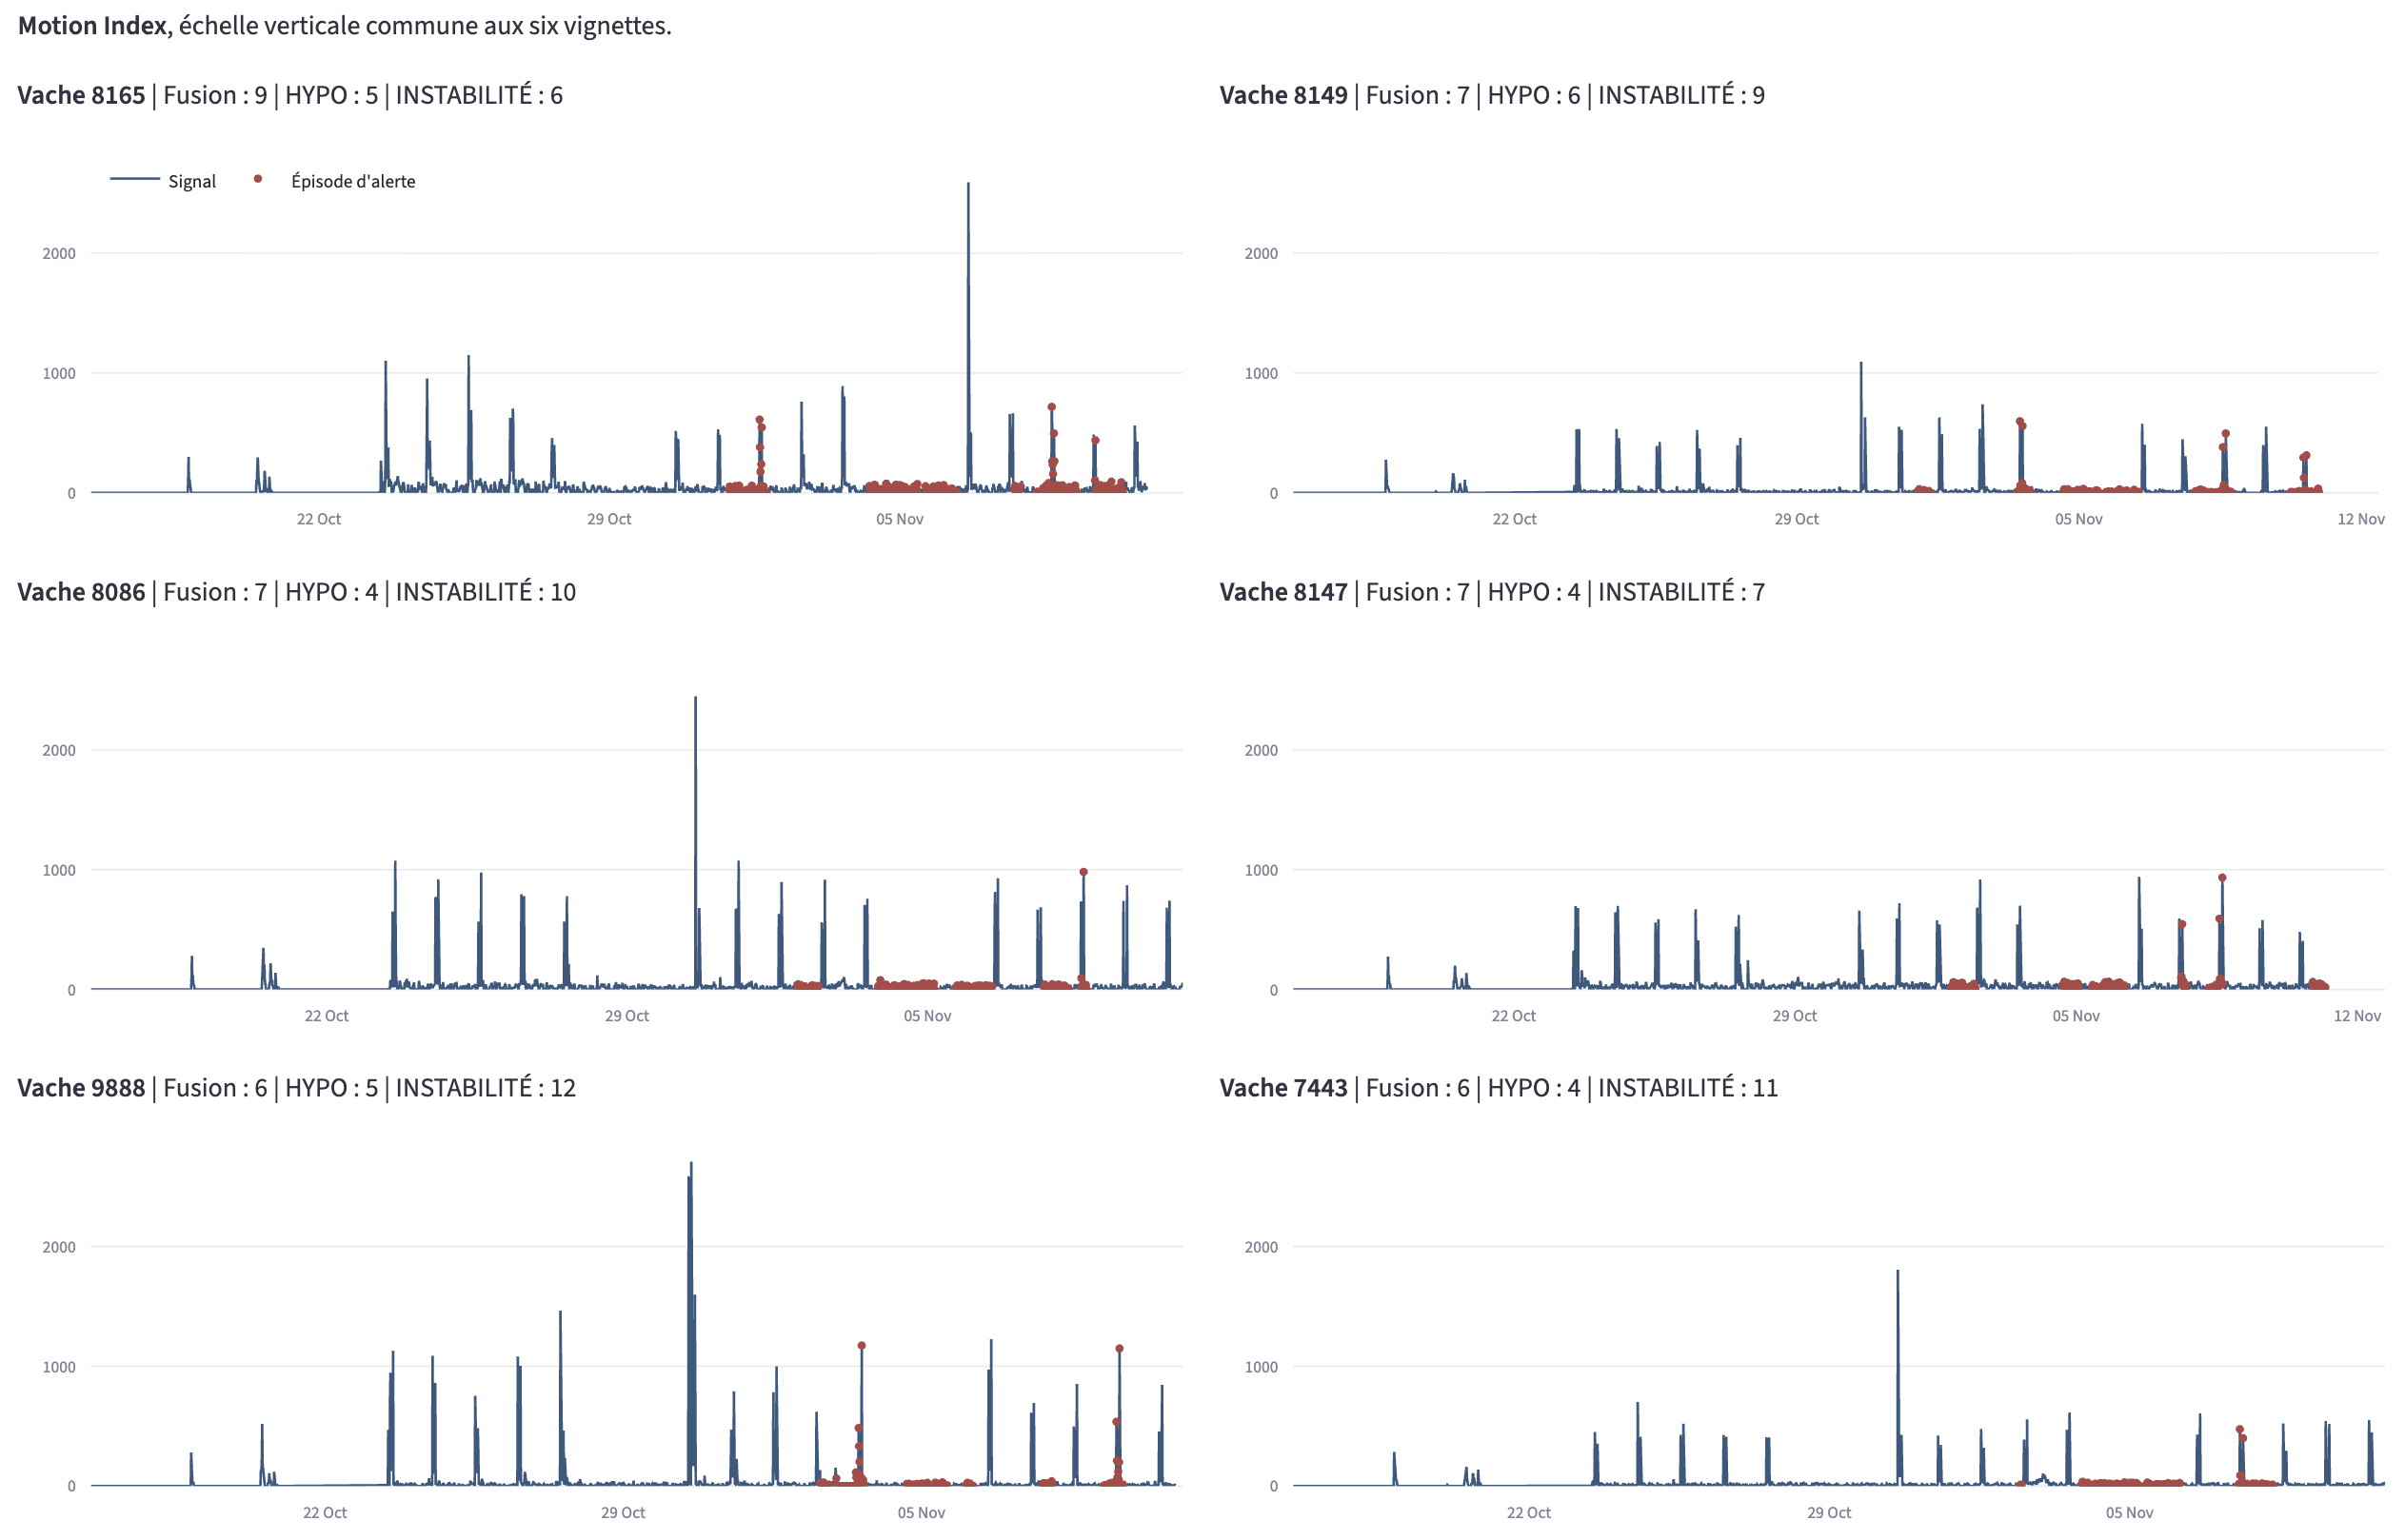
\includegraphics[width=0.96\linewidth]{figures/streamlit_priority_animals.png}
    \caption{Vaches à vérifier en priorité.}
    \label{fig:streamlit_priority_animals}
  \end{figure}
  \vfill
\end{landscape}

% =====================================================================
\section{Export et traçabilité des alertes}
% =====================================================================
Une priorité affichée n'a d'utilité que si elle peut sortir de l'écran. L'interface expose
donc un onglet d'export qui produit trois fichiers CSV~: un résumé par vache, les données
complètes du troupeau au grain de l'intervalle, et les alertes comportementales,
c'est-à-dire les débuts d'épisode retenus par la fusion. La vue individuelle permet en outre
d'exporter la série d'une vache telle qu'elle est affichée, avec les filtres appliqués. Ces fichiers
alimentent le registre d'élevage ou une vérification hors ligne, sans imposer que l'interface
reste ouverte.

La table individuelle et son export correspondent à la chaîne actuelle: épisodes et
notifications de la fusion, candidats HYPO, surveillance d'instabilité, couverture et
partition chronologique. Les sorties d'Isolation Forest y sont conservées uniquement comme
comparateur explicitement nommé. Les anciennes colonnes cliniques de la première chaîne ne
sont ni affichées ni exportées, afin qu'un résultat historique ne puisse être confondu avec
une sortie du système évalué dans ce mémoire. Le fichier CSV individuel contient exactement
les lignes visibles après application des filtres.

La traçabilité repose sur le nommage. Chaque fichier exporté porte la résolution temporelle
retenue et une empreinte courte du fichier source, calculée au chargement et affichée à
l'écran. L'export individuel y ajoute l'identifiant de la vache et la fenêtre de dates. Deux
exports issus de jeux de données ou de résolutions différents ne peuvent donc pas être
confondus, et un fichier retrouvé plusieurs semaines plus tard reste rattachable à son
origine. Cette empreinte sert à identifier une source, non à garantir son intégrité
cryptographique~: cette garantie relève du manifeste SHA-256 de la chaîne reproductible
(Annexe~\ref{annexe:validation}), dont ce nommage prolonge la logique à l'échelle de
l'interface.

% =====================================================================
\section{Portée et limites de l'usage en ferme}
% =====================================================================
L'interface est un prototype de démonstration. Elle s'exécute localement, charge un fichier
CSV et montre que les sorties du détecteur peuvent être lues, ordonnées et rattachées à des
vaches précises. Elle n'est pas un produit déployé~: elle ne gère ni l'acquisition continue
des mesures, ni les comptes utilisateurs, ni l'historique des vérifications réalisées.

L'usage prévu de l'interface est donc étroit, et cette étroitesse est assumée. Une priorité~3 signifie que
la vache mérite d'être regardée avant les autres, non qu'elle est boiteuse. Aucune vue
n'autorise à conclure à une boiterie sans examen du pied.

Une limite tient à l'évaluation de l'outil lui-même~: l'interface n'a pas été soumise à des
utilisateurs. Aucun éleveur ni technicien n'a été observé en train de s'en servir, et la
lisibilité des vues, le temps nécessaire pour trancher un cas et l'acceptabilité des
trois niveaux de priorité n'ont pas été mesurés. Les choix de présentation découlent du
positionnement du mémoire et des contraintes du détecteur, non d'une étude d'usage. Une
évaluation auprès d'utilisateurs réels constitue donc une étape nécessaire avant tout
déploiement, au même titre que la validation clinique du détecteur. La charge de vérification
que ce classement par priorité représente et ses conséquences pratiques pour l'éleveur sont examinées dans la
discussion générale.
